\documentclass[table,german,10pt]{beamer}
\usepackage[utf8]{luainputenc}
\usepackage{tcs-lecture}
\usepackage{yfonts}
\usepackage{nicefrac}
\usepackage{appendixnumberbeamer}

\usetikzlibrary{arrows, shapes}
\tikzstyle{edge} = [fill,opacity=.5,fill opacity=.5,line cap=round, line
join=round, line width=50pt]
% \input{../config/lecture-config.tex}

\DeclareMathOperator{\perm}{perm}
\DeclareMathOperator{\pcp}{PCP}
\DeclareMathOperator{\poly}{poly}
\DeclareMathOperator{\var}{Var}
\DeclareMathOperator{\longc}{Long}
\DeclareMathOperator{\twoponer}{2P1R}

\newcommand{\red}[1]{\textcolor{red}{#1}}
\newcommand{\blue}[1]{\textcolor{blue}{#1}}
\newcommand{\green}[1]{\textcolor{green!50!black}{#1}}
\newcommand{\purple}[1]{\textcolor{purple}{#1}}

\author{Sebastian Berndt}
\setbeamertemplate{sidebar right}{}
\setbeamertemplate{title page}
{
    

  \vbox{}
  \ifcd\vskip-5mm\leavevmode\hbox{\hskip-3mm\includegraphics[scale=0.45]{uzl-logo-ITCS.pdf}}%
  \par
  \leftskip3mm\else
  \vskip1em\fi
  {\huge \insertshortlecture\par}
  {\usebeamercolor[fg]{title}\usebeamerfont{title}\inserttitle\par}%
  \ifx\insertsubtitle\@empty%
  \else%
  \vskip0.25em%
  {\usebeamerfont{subtitle}\usebeamercolor[fg]{subtitle}\insertsubtitle\par}%
  \fi%     
  \vskip4pt\par
  \usebeamercolor[fg]{author}\insertauthor

}

\logo{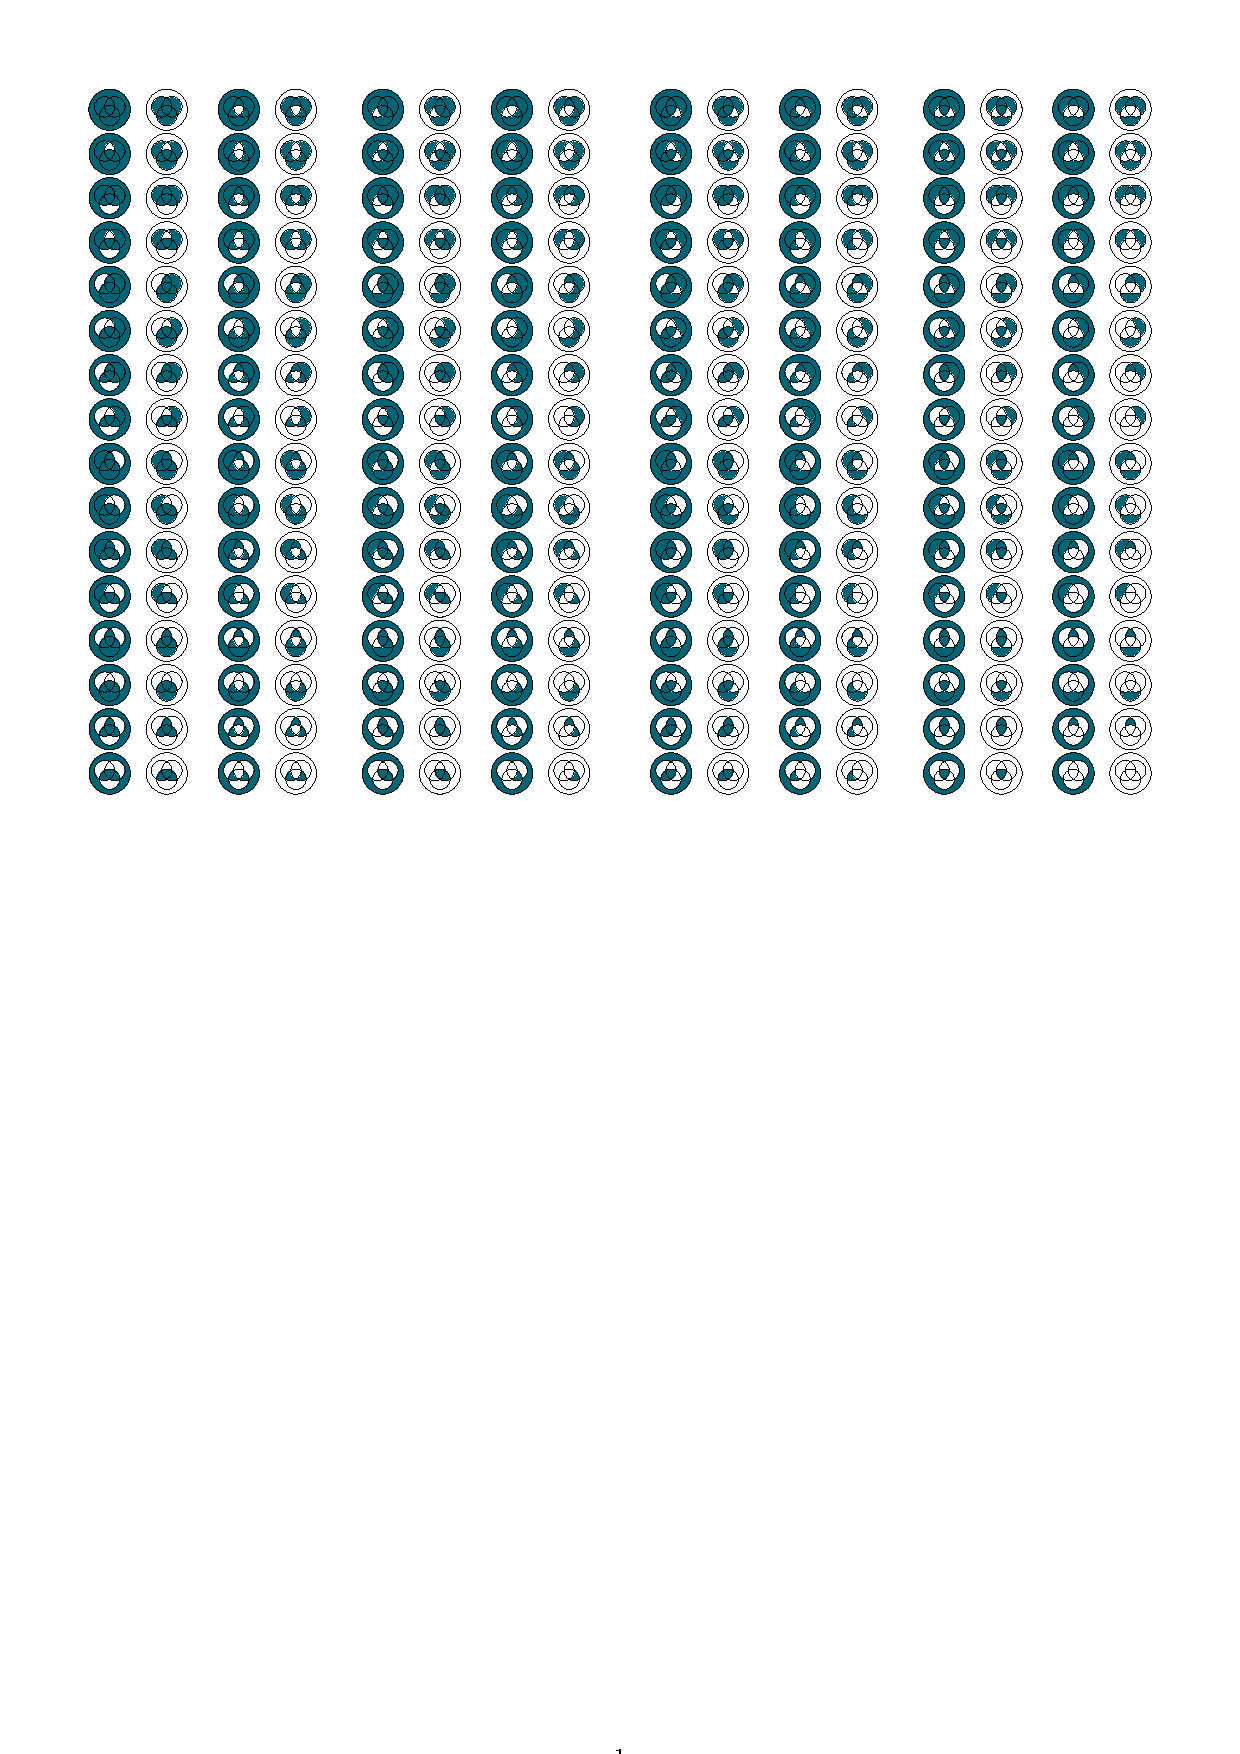
\includegraphics[scale=0.17]{logo}
}



\def\insertlecture{Oberseminar}
\lecture{PCP Teil 2}{in-ex}
\begin{document}


\maketitle

\begin{frame}{Heute}
  \begin{itemize}[<+->]
  \item Kurze Wiederholung
  \item Nicht-Approximierbarkeit von \textsc{max-3-lin}
  \item Unique Games Conjecture
  \item Nicht-Approximierbarkeit von \textsc{max-cut}
  \end{itemize}
\end{frame}
\begin{frame}{Wiederholung}
  \begin{block}{PCP}
    Die Klasse $\pcp_{\green{c},\purple{s}}[\red{r(n)},\blue{q(n)}]$ enthält alle Sprachen
    $\mathcal{L}\subseteq \{0,1\}^{*}$, für die es einen
    Verifier $V$ gibt mit:
    \begin{itemize}[<+->]
    \item $V$ erhält eine \emph{Instanz} $x\in \{0,1\}^{n}$ und einen
      \emph{Beweis} $\pi\in \{0,1\}^{*}$ (es reicht $|\pi|\leq
      2^{r(n)}\cdot q(n)$)
    \item $V$ läuft in Zeit $\poly(n)$
    \item $V$ darf $\mathcal{O}(\red{r(n)})$ Münzwürfe durchführen
    \item $V$ darf $\mathcal{O}(\blue{q(n)})$ Bits des Beweises $\pi$ lesen
    \item $\forall x\in \mathcal{L}: \exists \pi: \Pr[V^{\pi}(x)=1]\geq \green{c}$ (\emph{Completeness})
    \item $\forall x\not\in \mathcal{L}:\forall \pi:
      \Pr[V^{\pi}(x)=1]\leq \purple{s}$ (\emph{Soundness})

    \end{itemize}
  \end{block}
\end{frame}
\begin{frame}{Wiederholung}
  \begin{block}{PCP-Theorem (Arora, Lund, Motwani, Sudan, Szegedy)}
    \vspace{-0.5cm}
    \begin{align*}
      \pcp_{1,\nicefrac{1}{2}}[\log n,1]=\mathcal{NP}
    \end{align*}
  \end{block}
  \pause
  \begin{block}{\textsc{\epsilon-GAP-Max-3SAT}}
    \begin{description}
    \item[Gegeben:] \textsc{3SAT}-Formel $\varphi$ mit $m$ Klauseln
    \item[Gesucht:] 
      \begin{itemize}
      \item Ist $\varphi$ erfüllbar? (JA)
      \item Gilt für alle $\beta$, dass höchstens $(1-\epsilon)\cdot m$
        Klauseln gleichzeitig erfüllt sind? (NEIN)
      \end{itemize}
    \end{description}
    
  \end{block}
\pause
  \begin{block}{Nicht-Approximierbarkeit}
    Das PCP-Theorem ist äquivalent zur Aussage, dass es eine Konstante
    $\epsilon$ gibt, so dass \textsc{\epsilon-GAP-Max-3SAT}
    $\mathcal{NP}$-hart ist.
    
  \end{block}
  
\end{frame}

\begin{frame}{Allgemeines Vorgehen}
  \begin{enumerate}[<+->]
  \item Zeige, dass die Existenz eines bestimmten Verifiers $V^{*}$ die
    Nicht-Approximierbarkeit impliziert
  \item Baue einfachen Verifier $V$ (Outer Verifier)
  \item Modifiziere $V$ zu $V^{*}$ (Inner Verifier)
  \end{enumerate}
  
\end{frame}

% \begin{frame}{2P1R}
%   \begin{block}{\textsc{2P1R}}
%     $\mathcal{L}\in\twoponer_{\blue{c},\green{s}}[\red{r(n)}]$ gdw. es
%     gibt polynomiellen Algorithmus $W$ mit $\mathcal{O}(\red{r(n)})$
%     Münzwürfen, der zwei Fragen $q_{1},q_{2}$ an zwei Prover
%     $P_{1},P_{2}$ schickt, so dass:
%     \begin{itemize}
%     \item $\forall x\in \mathcal{L}:\exists P_{1},P_{2}$: Die Antworten
%       $P_{1}(q_{1}),P_{2}(q_{2})$ führen mit Wahrscheinlichkeit $\blue{c}$ zur
%       Akzeptanz von $W$
%     \item $\forall x\not\in \mathcal{L}: \forall P_{1},P_{2}$: Die
%       Antworten $P_{1}(q_{1}),P_{2}(q_{2})$ führen höchstens mit
%       Wahrscheinlichkeit $\green{s}$ zur Akzeptanz
%     \end{itemize}
%     $P_{1}$ und $P_{2}$ dürfen \emph{nicht miteinander
%       kommunizieren}. Ihre Antworten müssen ``\emph{konsistent}'' sein.
%   \end{block}
% \pause
% \begin{block}{Idee}
%   \begin{itemize}[<+->]
%   \item $W$ kann nur $2^{r(n)}$ Fragen stellen
%   \item Schreibe diese als Beweis $\pi$ auf
%   \item Erhalte so PCP
%   \end{itemize}
% \end{block}
% \end{frame}
% \begin{frame}{CSP}
%   \begin{block}{\textsc{CSP}}
%     \begin{description}
%     \item[Gegeben:] Variablen $\var$, Domain $D$, Constraints $C=\{\langle
%       t_{1},R_{1}\rangle,\langle t_{2},R_{2}\rangle,\ldots\}$ mit
%       $t_{i}\in \var^{2}, R_{i}\in D^{2}$
%     \item[Gesucht:] Gibt es eine Abbildung $f\colon\var\to D$ mit
%       $(f(x),f(x'))\in R$ für alle $\langle (x,x'),R\rangle\in C$?
%     \end{description}
%   \end{block}
% \pause
% \begin{block}{Beispiel}
% 3-Färbbarkeit:
% \begin{itemize}[<+->]
% \item $\var=V$
% \item $D=\{1,2,3\}$
% \item Constraints $\langle
%   (v,w),\{(1,2),(1,3),(2,1),(2,3),(3,1),(3,2)\}\rangle$ für alle
%   $\{v,w\}\in E$
% \end{itemize}
% \end{block}
  
%\end{frame}
\begin{frame}{Label Cover}
  \begin{block}{\textsc{Label-Cover}}
    \begin{description}
    \item[Gegeben:] Bipartiter, regulärer Graph $G=(X\dot{\cup} Y, E)$,
      Alphabete $\Sigma_{X},\Sigma_{Y}$, Menge von $\Pi=\{\pi_{e}\colon
      \Sigma_{X}\to \Sigma_{Y} \mid e\in E\}$
    \item[Gesucht:] Zwei Abbildungen $\ell_{X}\colon X\to \Sigma_{X},
      \ell_{Y}\colon Y\to \Sigma_{Y}$, so dass für
      alle $(x,y)\in E$ gilt $\pi_{(x,y)}(\ell_{X}(x))=\ell_{Y}(y)$. 
    \end{description}
    
  \end{block}
  \pause
  \begin{block}{Beispiel}
    3SAT-Formel $\varphi=\bigwedge_{i=1}^{m}K_{i}$ mit Variablen $x_{1},\ldots,x_{n}$

    \begin{itemize}[<+->]
    \item $X=\{K_{1},K_{2},\ldots,K_{m}\}$
    \item $Y=\{x_{1},x_{2},\ldots,x_{n}\}$
    \item $E=\{(K,x)\mid x\in K\}$
    \item $\Sigma_{X}=[1..7]$
    \item $\Sigma_{Y}=\{0,1\}$
    \item $\pi_{(K,x)}$ wandelt Belegung von $K$ in Belegung von $x$ um 
    \end{itemize}
  \end{block}
\pause
\begin{theorem}
  Es gibt eine Konstante $\epsilon'$, so dass
  \textsc{\epsilon'-GAP-Max-Label-Cover} $\mathcal{NP}$-hart ist.
\end{theorem}
  
\end{frame}

\begin{frame}{\textsc{3-lin}}
  \begin{block}{\textsc{3-lin}}
  \begin{description}
  \item[Gegeben:] Menge von Variablen $x_{1},\ldots,x_{n}$ und
    Gleichungen $C$ der Form $x\oplus y\oplus z=\{0,1\}$
  \item[Gesucht:] Belegung $\beta\colon\{x_{1},x_{2},\ldots,x_{n}\}\to
    \{0,1\}$, so dass alle Gleichungen erfüllt sind
  \end{description}
  \end{block}  
\pause
\begin{theorem}[Johan Håstad, 2001]
  Wenn es einen $(\log n,1)$-Verifier $V$ mit Soundness $s$ und
  Completeness $c$ gibt, der genau drei Bits $x,y,z$ liest und
  akzeptiert, falls $x\oplus y\oplus z=0$, so kann \textsc{max-3-lin} nicht besser
  als mit Rate $\nicefrac{s}{c}$ approximiert werden. (außer
  $\mathcal{P}=\mathcal{NP}$)
\end{theorem}
\pause
\begin{block}{Beweis}
  \begin{itemize}[<+->]
  \item Variablen $x_{1},x_{2},\ldots$
  \item Simuliere Münzwürfe und konstruiere Gleichungen $C=\{
    x_{i}\oplus x_{j} \oplus x_{k}=0\mid \Pr[\text{$V$ liest gleichzeitig Bits
      $i,j,k$}]>0\}$
  \item $\Pr[\text{$V$ akzeptiert}]=\frac{\text{Anzahl erfüllter
        Gleichungen}}{\text{Anzahl der Gleichungen}}$
  \end{itemize}
\end{block}

\end{frame}
\begin{frame}{Outer Verifier}
\textsc{label-cover} Instanz
      $G=(X\dot{\cup}Y,E),\Sigma,\Pi=\{\pi_{e}\}_{e\in E}$

Konstruiere typischen Verifier für \textsc{label-cover}:

\pause
\begin{block}{Verifier}
  

\begin{itemize}[<+->]
\item Wähle $(x,y)\in E$ uniform
\item Lies $\ell_{X}(x),\ell_{Y}(y)$ aus dem Beweis
\item Teste, ob $\pi(\ell_{X}(x))=\ell_{Y}(y)$ 
\end{itemize}
\end{block}

\pause
Wenn alle Kanten erfüllt sind, ist die
Wahrscheinlichkeit, dass diese erfüllt ist, $1$.
\pause

Sind maximal $(1-\epsilon)\cdot |E|$ der Kanten erfüllt, ist die
Wahrscheinlichkeit, dass diese erfüllt ist, höchstens $(1-\epsilon)$. 

\pause
\red{Wir lesen $\log|\Sigma_{X}|+\log|\Sigma_{Y}|$ Bits!}

  
\end{frame}

  \begin{frame}{3-Bit Verifier / Inner Verifier}
  \begin{block}{Idee}
    Wir codieren $\ell_{X}(x),\ell_{Y}(y)$ so, dass wir für den Test
    $\pi(\ell_{X}(x))=\ell_{Y}(y)$ nur drei Bits lesen müssen!
  \end{block}
\pause
\begin{block}{Long Code}
  Sei $\mathcal{B}_{\Sigma}=\{f\colon\Sigma\to \{0,1\}\}$ Menge der booleschen
  Funktionen ($|\mathcal{B}_{\Sigma}|=2^{|\Sigma|}$) mit
  $\mathcal{B}_{\Sigma}=\{f_{0},f_{1},\ldots,f_{2^{|\Sigma|}-1}\}$. 

  Wir codieren $a\in \Sigma$ mit $\longc_{a}=f_{0}(a)f_{1}(a)\ldots
  f_{2^{|\Sigma|}-1}(a)$, d.h. $\longc_{a}[f]=f(a)$ für alle $f\in \mathcal{B}_{\Sigma}$.
  
\end{block}
\end{frame}

  \begin{frame}{3-Bit Verifier / Inner Verifier}
    Neuer 3-Bit Verifier:
    \begin{block}{Verifier}
    \begin{itemize}[<+->]
    \item Wähle zufällig $(x,y)\in E$
    \item Wähle zufällig $f\in B_{\Sigma_{X}},g\in B_{\Sigma_{Y}}$, mit
      $\Pr[f(\sigma)=1]=\nicefrac{1}{2}=\Pr[g(\sigma')=1]$
    \item Teste, ob
      $\longc_{\ell_{X}(x)}[f]\oplus \longc_{\ell_{Y}(y)}[g]\oplus \longc_{\ell_{X}(x)}[(g\circ
      \pi_{(x,y)})\oplus f]=0$
    \end{itemize}
    \end{block}

\pause
\begin{block}{Completeness}
Falls $\pi(\ell_{X}(x))=\ell_{Y}(y)$:
\pause
\begin{block}{Soundness}
Idee: Wenn der Test mit zu hoher Wahrscheinlichkeit gelingt, gibt uns
$\longc_{\ell}$ ein Labeling, dass sehr viele Kanten erfüllt.

Beweis: Fourier-Analyse von $\longc_{\ell}$

\end{block}
  
\end{block}
  \end{frame}
  \begin{frame}{Konsequenzen}

    \begin{theorem}
      Wir erhalten $c=1-\epsilon, s=\nicefrac{1}{2}+\epsilon$. Eine
      bessere Approximation als $2-\epsilon$ ist nicht möglich!
    \end{theorem}
\pause

    Weiteres Fortführen der Ideen:

    \begin{theorem}[Johan Håstad, 2001]
      Es gibt keinen Algorithmus, der \textsc{max-3SAT} besser als mit
      Rate $\nicefrac{8}{7}$ approximieren kann. (außer $\mathcal{P}=\mathcal{NP}$)
    \end{theorem}
    
  \end{frame}

\begin{frame}{Allgemeines Vorgehen}
  \begin{enumerate}[<+->]
  \item Zeige, dass die Existenz eines bestimmten Verifiers $V^{*}$ die
    Nicht-Approximierbarkeit impliziert
  \item Baue einfachen Verifier $V$ (Outer Verifier)
  \item Modifiziere $V$ zu $V^{*}$ (Inner Verifier)
  \end{enumerate}
  
\end{frame}

% \begin{frame}{\textsc{label-cover} $\in \twoponer$}
% \begin{block}{Theorem}
%   \textsc{Label-cover} $\in \twoponer_{\blue{1},\green{1-\nicefrac{1}{|E|}}}[\log n]$
% \end{block}
% \pause
% \begin{block}{Beweis}
%   \begin{itemize}[<+->]
%   \item $G=(X\dot{\cup}Y,E), \Sigma, \Pi=\{\pi_{e}\}_{e\in E}$ Instanz von
%     \textsc{Label-cover}
%   \item Wähle zufällig $(x,y)\in E$ und frage $P_{1}$ nach $\ell(x)$ und
%     $P_{2}$ nach $\ell(y)$
%   \item Erfüllbar: $P_{1}$ und $P_{2}$ wählen gültige Abbildung, also \blue{$c=1$}
%   \item Nicht-erfüllbar: Jede Abbildung erfüllt mind. eine Kante nicht,
%     also \green{$s=1-\nicefrac{1}{|E|}$}
%   \end{itemize}  
% \end{block}
% \pause
% \begin{block}{Konsequenz}
% Zwei Sichtweisen: Entweder Optimierungsproblem oder Spiel
% \end{block}
% \end{frame}
\begin{frame}{Unique Games}
  \begin{block}{\textsc{unique-label-cover}}
      Sei $G=(X\dot{\cup}Y,E),\Sigma,\Pi=\{\pi_{e}\}_{e\in E}$ Instanz
      von \textsc{label-cover}. Sind alle $\pi_{e}$ Permutationen, so
      ist es eine Instanz von \textsc{unique-label-cover}. 
  \end{block}
  \pause
  \begin{block}{Frage}
    Wie schwer ist \textsc{unique-label-cover}?
  \end{block}
  \pause
  \begin{block}{\textsc{\epsilon-GAP-Max-unique-label-cover}}
    \begin{description}
    \item[Gegeben:] \textsc{unique-label-cover} Instanz
      $G=(X\dot{\cup}Y,E),\Sigma,\Pi=\{\pi_{e}\}_{e\in E}$
    \item[Gesucht:] 
      \begin{itemize}
      \item Sind mindestens $(1-\epsilon)\cdot |E|$ Kanten erfüllbar? (JA)
      \item Gilt für alle $\ell$, dass höchstens $\epsilon\cdot |E|$
        Kanten gleichzeitig erfüllt sind? (NEIN)
      \end{itemize}
    \end{description}
  \end{block}
  \pause
  \begin{block}{Unique Games Conjecture (Subhash Khot, 2002)}
    Für alle $\epsilon>0$ gibt es ein $s=s(\epsilon)$, so dass
    \textsc{\epsilon-GAP-Max-unique-label-cover} $\mathcal{NP}$-hart für
    Instanzen mit Alphabetgröße $s$ ist. 
    
  \end{block}
  
\end{frame}
\begin{frame}{Unique Games Conjecture}
    Zustand 2005:
    
  \begin{table}
    \centering

    \begin{tabular}{|c|c|c|c|}
      Name & Rate & LB & LB UGC\\
      \textsc{min-vertex-cover} & 2 & 1{.}36 & $2-\epsilon$\\
      \textsc{max-cut} & $\nicefrac{1}{\alpha_{GW}}\approx 1{.}139$ &
      $\nicefrac{17}{16}\approx 1.0625$ & $\nicefrac{1}{\alpha_{GW}}-\epsilon$\\
      \textsc{min-k-uniform-hypergraph-vc} & $k$ & $k-1-\epsilon$ & $k-\epsilon$\\
      \textsc{max-2SAT} & $\nicefrac{1}{\alpha_{LLZ}}\approx 1{.}064$ &
      $1{.}048$ & $\nicefrac{1}{\alpha_{LLZ}}-\epsilon$\\
      \textsc{CSP} mit integrality gap $\alpha$ & $\alpha$ & ? & $\alpha-\epsilon$
    \end{tabular}
  \end{table}

\pause

\begin{theorem}[Raghavendra, 2008]
  Unter der UGC ist jedes CSP entweder $\mathcal{NP}$-hart oder in
  Polynomialzeit lösbar.
\end{theorem}
  
\end{frame}
\begin{frame}{Ein Beispiel}
  \begin{block}{\textsc{max-cut}}
    \begin{description}
    \item[Gegeben:] Graph $G=(V,E)$
    \item[Gesucht:] Partition $V=V_{1}\dot{\cup} V_{2}$, so dass die
      Anzahl an Kanten zwischen $V_{1}$ und $V_{2}$ maximal ist.
    \end{description}
  \end{block}
\pause
\begin{theorem}[Khot, Kindler, Mossel, O'Donnel, 2005]
  Wenn es einen $(\log n,1)$-Verifier $V$ gibt mit Soundness $s$ und
  Completeness $c$ gibt, der genau zwei Bits $b,b'$ liest und
  akzeptiert, falls $b\neq b'$, so impliziert die UGC, dass
  \textsc{max-cut} nicht besser als mit Wert $\nicefrac{s}{c}$
  approximiert werden kann.
\end{theorem}
\pause
\begin{block}{Beweis}
  \begin{itemize}[<+->]
  \item $\pi$ Beweis für $V$
  \item Konstruiere $G=(V,E)$
  \item $V=\{v_{1},v_{2},\ldots,v_{|\pi|}\}$
  \item $E=\{(v_{i},v_{j})\mid \Pr[\text{$V$ liest Bits $i$ und $j$}]>0\}$
  \item $\Pr[\text{$V$ akzeptiert}]=\frac{\text{Anzahl der Kanten im
        Cut}}{\text{Anzahl der Kanten}}$

  \end{itemize}

  
\end{block}
\end{frame}
\begin{frame}{Outer Verifier}
\textsc{unique-label-cover} Instanz
      $G=(X\dot{\cup}Y,E),\Sigma,\Pi=\{\pi_{e}\}_{e\in E}$

Konstruiere typischen Verifier für \textsc{unique-label-cover}:

\pause
\begin{block}{Verifier}
\begin{itemize}[<+->]
\item Wähle $x\in X$ uniform
\item Wähle zufällig $(x,y),(x,y')\in E$
\item Sei $\pi=\pi_{(x,y)},\pi'=\pi_{(x,y')}$
\item Lies $\ell(x),\ell(y),\ell(y')$ aus dem Beweis
\item Teste, ob $\pi(\ell(x))=\ell(y)$ und $\pi'(\ell(x))=\ell(y')$

\end{itemize}
\end{block}

\pause
Wenn $(1-\epsilon)\cdot |E|$ der Kanten erfüllt, ist die
Wahrscheinlichkeit, dass beide erfüllt sind, mindestens $1-2\epsilon$. 
\pause

Sind maximal $\epsilon\cdot |E|$ der Kanten erfüllt, ist die
Wahrscheinlichkeit, dass beide erfüllt sind, höchstens $\epsilon$. 

\pause
\red{Wir lesen $3\cdot \log(|\Sigma|)$ Bits!}
  
\end{frame}

\begin{frame}{2-Bit Verifier / Inner Verifier}
  \begin{block}{Idee}
    Wir codieren  $\ell(x),\ell(y),\ell(y')$ so, dass wir für den Test
    $\pi(\ell(x))=\ell(y)$ und $\pi'(\ell(x))=\ell(y')$ nur zwei Bits
    lesen müssen!
  \end{block}
  \pause

  Auch hier wieder Long Code!
\end{frame}
\begin{frame}{2-Bit Verifier / Inner Verifier}
\begin{block}{Verifier mit Parameter $0<\rho<1$}
  \begin{itemize}[<+->]
\item Wähle $x\in X$ uniform
\item Wähle zufällig $(x,y),(x,y')\in E$
\item Sei $\pi=\pi_{(x,y)}^{-1},\pi'=\pi_{(x,y')}^{-1}$
  \item Wähle $f\in B_{|\Sigma|}$, so dass $\Pr[f(\sigma)=0]=\nicefrac{1}{2}$
  \item Wähle $f_{\rho}\in B_{|\Sigma|}$, so dass $\Pr[f_{\rho}(\sigma)=0]=\nicefrac{1}{2}+\nicefrac{1}{2}\rho>\nicefrac{1}{2}$
  \item Teste, ob $\longc_{\ell(y)}[f\circ
    \pi]=\longc_{\ell(y')}[(f\circ \pi')\cdot f_{\rho}]$
  \end{itemize}
  
\end{block}
\pause
\begin{block}{Completeness}
  Falls $\pi(\ell(x))=\ell(y)$ und $\pi'(\ell(x))=\ell(y')$:
\end{block}
\pause
\begin{block}{Soundness}
Idee: Wenn der Test mit zu hoher Wahrscheinlichkeit gelingt, gibt uns
$\longc_{\ell}$ ein Labeling, dass sehr viele Kanten erfüllt. 

Beweis: Fourier-Analyse von $\longc_{\ell}$ und ``Majority is Stablest''
  
\end{block}
  
\end{frame}
\begin{frame}{Konsequenzen}
  \begin{theorem}
    Wir erhalten $c=\nicefrac{1}{2}+\nicefrac{1}{2}\rho$ und
    $s=\nicefrac{\arccos(\rho)}{\pi}+\epsilon$. Eine bessere
    Approximation als $\nicefrac{s}{c}\approx
    \nicefrac{1}{\alpha_{GW}}-\epsilon\approx 1{.}139-\epsilon$ ist
    nicht möglich. ($\alpha_{GW}=\min_{0<\Theta\leq \pi}
    \frac{2}{\pi}\cdot \frac{\Theta}{1-\cos \Theta}$)
  \end{theorem}
  \pause
    \begin{theorem}[Goemans \& Williamson, 1995]
      Es gibt einen \emph{randomisierten} Approximationsalgorithmus für
      $\textsc{max-cut}$ mit Approximationsrate
      $\nicefrac{1}{\alpha_{GW}}\approx 1{.}139$.
    \end{theorem}
    \pause
    \begin{theorem}[Mahajan, Ramesh, 1995]
      Es gibt einen \emph{deterministischen} Approximationsalgorithmus
      für $\textsc{max-cut}$ mit Approximationsrate
      $\nicefrac{1}{\alpha_{GW}}\approx 1{.}139$.
    \end{theorem}

  
\end{frame}
\begin{frame}{Allgemeines Vorgehen}
  \begin{enumerate}[<+->]
  \item Zeige, dass die Existenz eines bestimmten Verifiers $V^{*}$ die
    Nicht-Approximierbarkeit impliziert
  \item Baue einfachen Verifier $V$ (Outer Verifier)
  \item Modifiziere $V$ zu $V^{*}$ (Inner Verifier)
  \end{enumerate}
  
\end{frame}

\end{document}









